% !TEX root = ./arock_pkg_main.tex
\subsection{Minimizing Elastic Net Logistic Regression}
In this subsection, we apply ARock with FBS to the elastic net regularized logistic regression problem
\begin{equation}\label{eqn:l12_log}
\Min_{x \in \mathbb{R}^n} \lambda_1 \|x\|_1 + \frac{\lambda_2}{2} \|x\|^2_2 + \sum_{i=1}^N \log\big(1 + \exp(-b_i \cdot a_i^T x)\big),
\end{equation}
where $\{(a_i, b_i)\}_{i=1}^N$ is the set of sample-label pairs, $\lambda_1=0.001$, $\lambda_2 = 1.$, and $n$ and $N$ represent the numbers of features and samples, respectively. This test uses two libsvm datasets\footnote{\url{http://www.csie.ntu.edu.tw/~cjlin/libsvmtools/datasets/}}: news20, and url.

Figure \ref{fig:log_reg_obj} gives the running times of  the full update (sync-parallel) and ARock (async-parallel) implementations on the two datasets. Figure~\ref{fig:log_reg_speedup} is the speedup performance comparison of the two methods. We can observe that ARock achieves approximate-linear speedup, but sync-parallel scales poorly as we explain below. One can also see that ARock converges faster due to more relaxed forward operator step size selection.

\begin{figure}[!h]
        \centering
       \begin{subfigure}[b]{0.4\textwidth}
                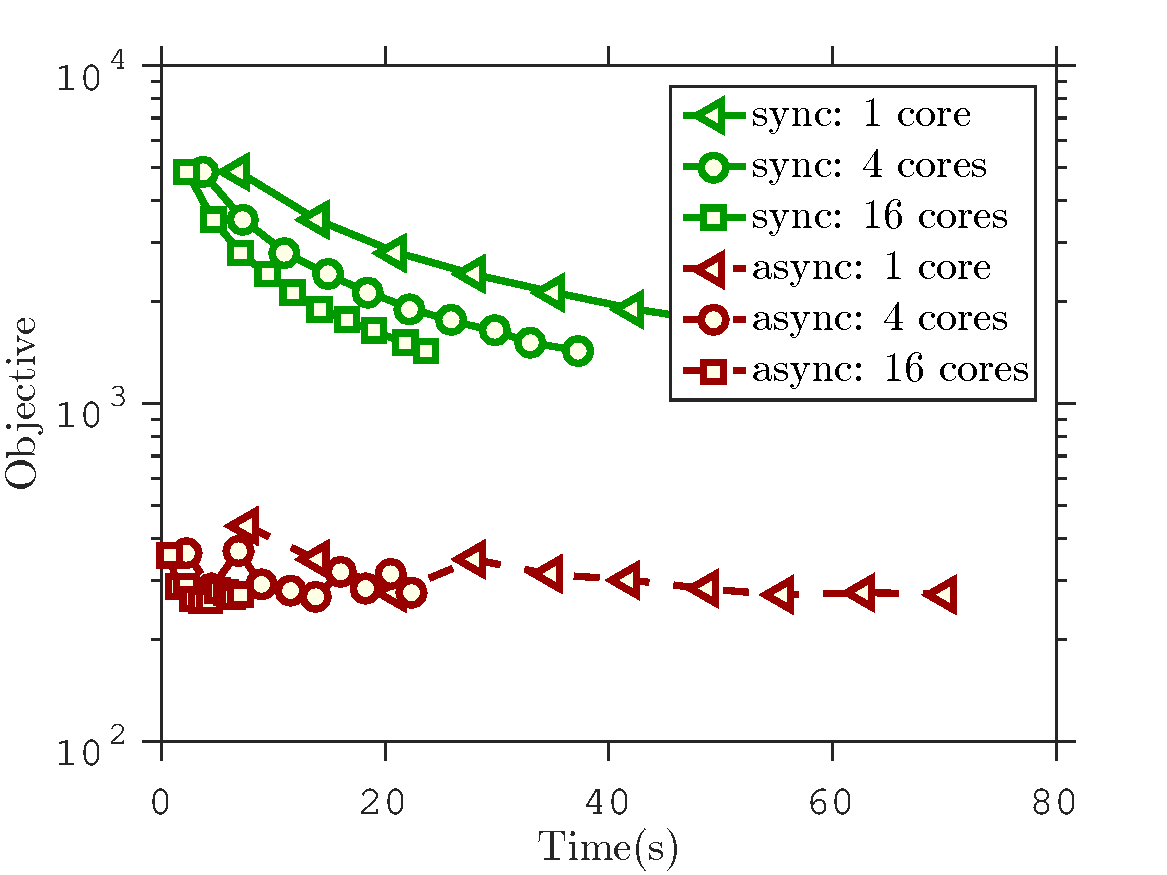
\includegraphics[width=\textwidth]{./figs/news20_obj}
                \caption{news20}
        \end{subfigure}
        ~~
        \begin{subfigure}[b]{0.4\textwidth}
                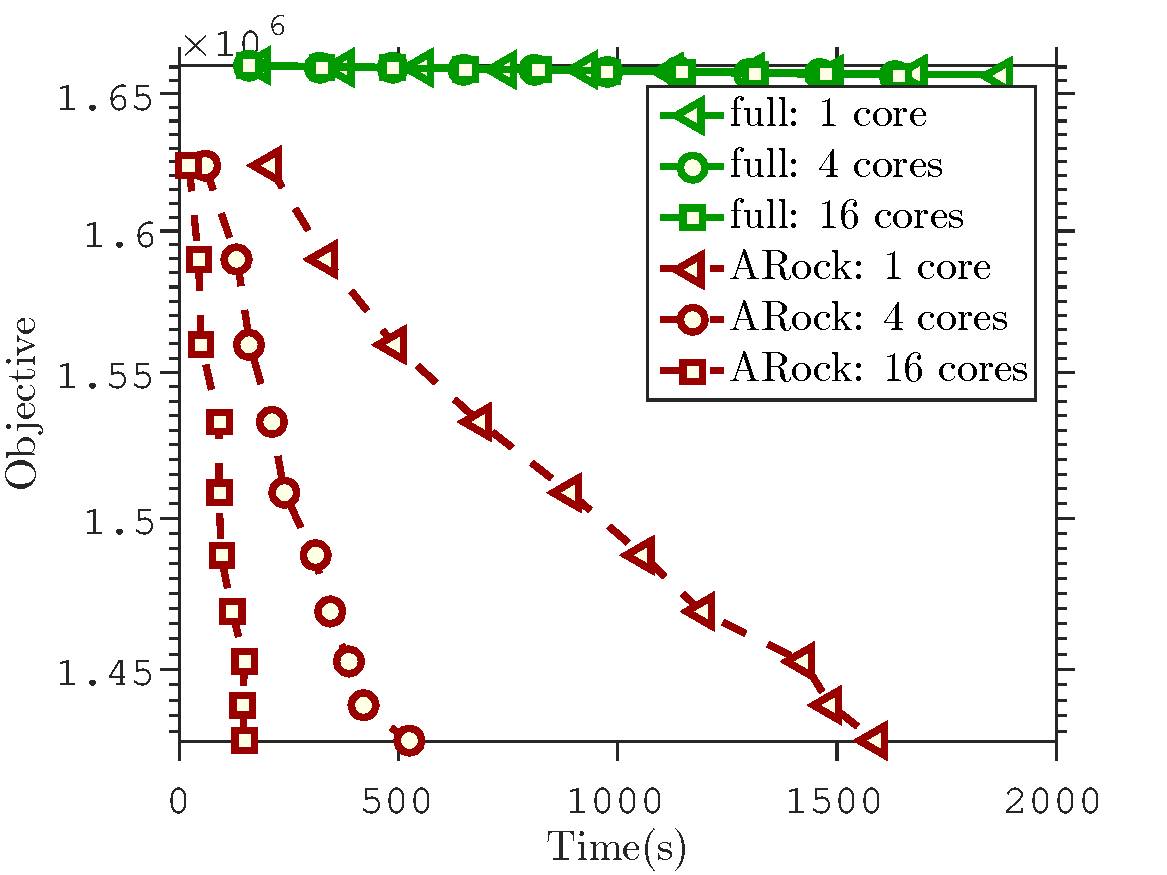
\includegraphics[width=\textwidth]{./figs/url_obj}
                \caption{url}
        \end{subfigure} 
        \caption{Objective vs wall clock time.}\label{fig:log_reg_obj}
\end{figure}

\begin{figure}[!h]
        \centering
       \begin{subfigure}[b]{0.35\textwidth}
                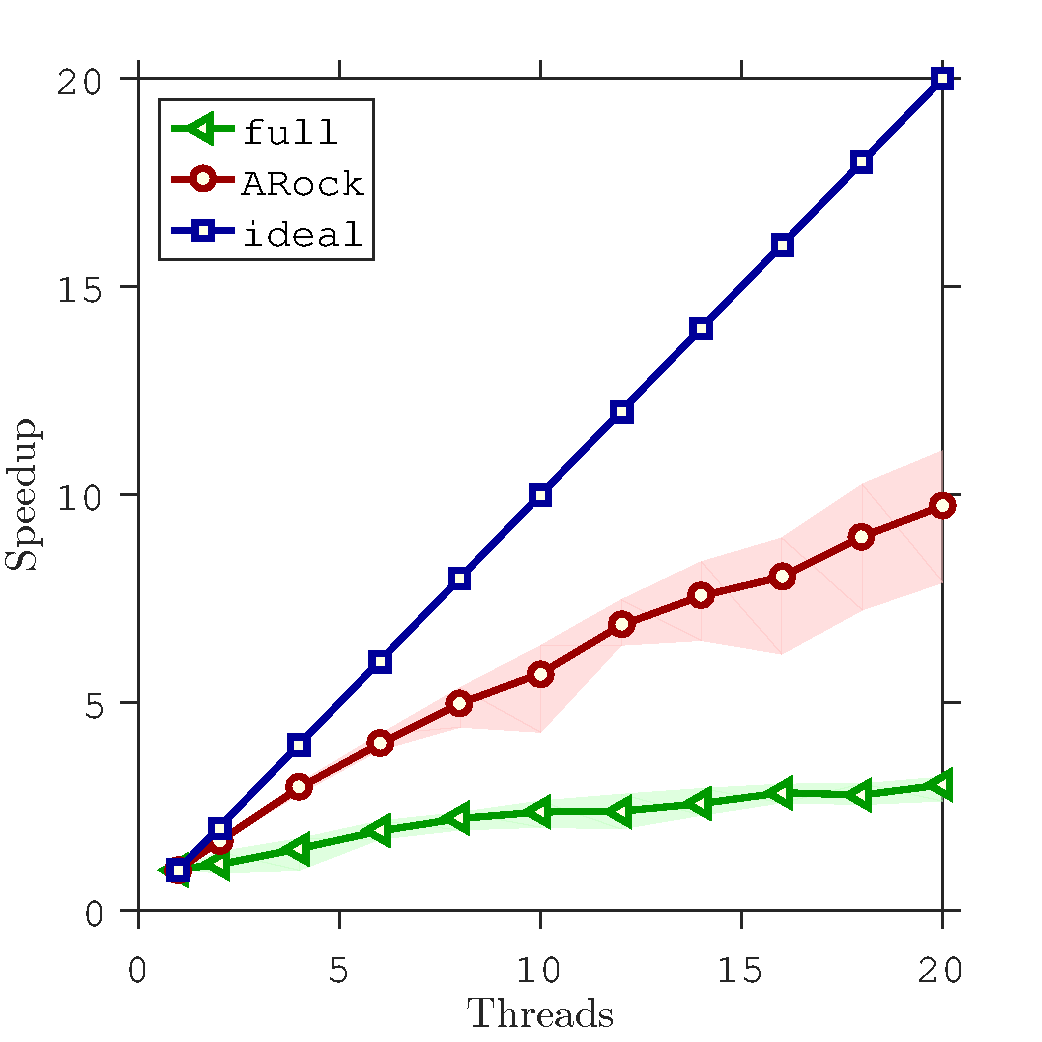
\includegraphics[width=\textwidth]{./figs/news20_speedup}
                \caption{news20}
        \end{subfigure}
        ~~
        \begin{subfigure}[b]{0.35\textwidth}
                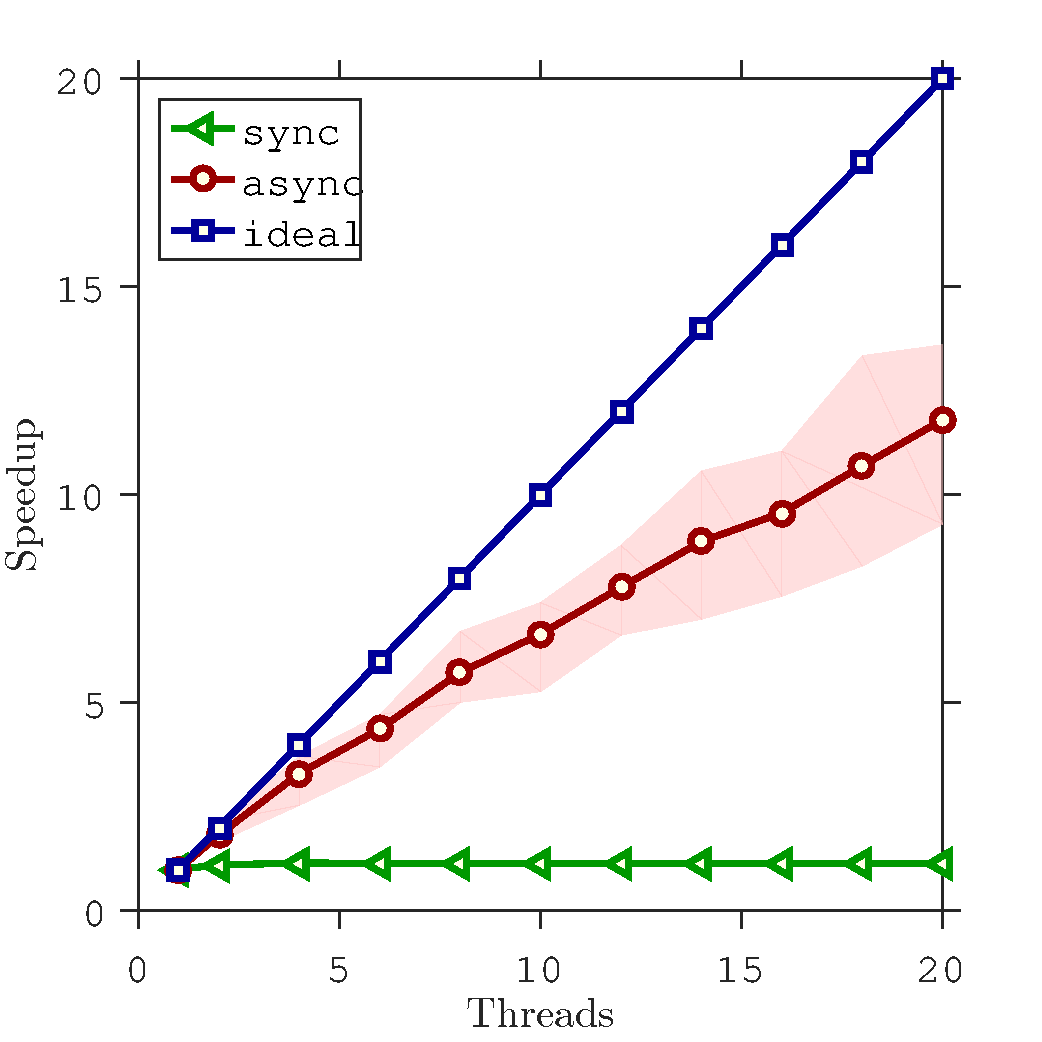
\includegraphics[width=\textwidth]{./figs/url_speedup}
                \caption{url}
        \end{subfigure}        
        \caption{Speedup vs number of threads.}\label{fig:log_reg_speedup}
\end{figure}
